%%%% fatec-article.tex, 2024/03/10

%% Classe de documento
\documentclass[
  a4paper,%% Tamanho de papel: a4paper, letterpaper (^), etc.
  12pt,%% Tamanho de fonte: 10pt (^), 11pt, 12pt, etc.
  english,%% Idioma secundário (penúltimo) (>)
  brazilian,%% Idioma primário (último) (>)
]{article}

%% Pacotes utilizados
\usepackage{float}
\usepackage[]{fatec-article}
\Author{1}{Name={Samia Muniz Braz \\ Catarine Pereira da Silva\\ Marcelo Augusto Pedroso Martins}}

\Author{2}{Name={\{ samia.braz@fatec.sp.gov.br \}\\ \{ Catarine.silva@fatec.sp.gov.br \} \\ \{ marcelo.martins36@fatec.sp.gov.br\} }}

%% Definição das palavras-chaves/keywords
\Keyword{1}{Agricultura}{Agriculture}
\Keyword{2}{Deep Learning}{Deep Learning}
\Keyword{3}{Gomose}{Gummosis}
\Keyword{4}{Citros}{Citrus}
\Keyword{5}{Visão Computacional}{Computer Vision}




%%%% Resumo no idioma primário (brazilian)
\begin{Abstract}[brazilian]%% Idioma (brazilian ou english)
  O Brasil é o país mais produtor de laranja e também o maior exportador de suco de acordo com A Secretaria de Comércio Exterior (Secex/MDIC) , representando 75 porcento do mercado global da bebida, a produção de citros se encontra no estado de São Paulo, com um pomar de 183.783.180 plantas cítricas (DEFESA AGROPECUÁRIA ESTADO DE SÃO PAULO, 2015). O Brasil como maior produtor do citros enfrenta um fungo que impacta na produtividade e na exportação do citros e que causa a morte das plantas assim surgindo a necessidade do replantio das plantas nos pomares, o fungo do gênero Phytophthora chamado gomose, também conhecido como podridão do pé, ataca as plantas jovens nos pomares que estão em produção e provoca danos ao seu tronco, com a degradação das raízes e radicelas. Surge então a necessidade da criação de uma identificação rápida da doença para o tratamento contra a gomose ser mais eficaz, o aplicativo criado visa identificar a doença com Inteligência Artificial (IA) por meio de Redes Neurais Artificiais.
\end{Abstract}

%%%% Resumo no idioma secundário (english)
\begin{Abstract}[english]%% Idioma (brazilian ou english)
  Brazil is the largest orange producing country and also the largest exporter of juice according to the Secretariat of Foreign Trade (Secex/MDIC), representing 75 percent of the global beverage market, citrus production is found in the state of São Paulo , with an orchard of 183,783,180 citrus plants (DEFESA AGROPECUÁRIA ESTADO DE SÃO PAULO, 2015). Brazil, as the largest producer of citrus, faces a fungus that impacts the productivity and export of citrus and causes the death of plants, resulting in the need to replant plants in orchards, the fungus of the genus Phytophthora called gummosis, also known as citrus rot. standing, attacks young plants in orchards that are in production and causes damage to their trunk, with the degradation of roots and radicelles. The need then arises to create a rapid identification of the disease for the treatment against gummosis to be more effective. The application created aims to identify the disease with Artificial Intelligence (AI) through Artificial Neural Networks.
\end{Abstract}

%% Processamento de entradas (itens) do índice remissivo (makeindex)
\makeindex%

%% Arquivo(s) de referências
\addbibresource{fatec-article.bib}

%% Início do documento
\begin{document}

% Seções e subseções
%\section{Título de Seção Primária}%

%\subsection{Título de Seção Secundária}%

%\subsubsection{Título de Seção Terciária}%

%\paragraph{Título de seção quaternária}%

%\subparagraph{Título de seção quinária}%

\section*{Introdução}
A doença gomose têm um impacto considerável na produção de citros no Brasil, já que, o cultivo dessas frutas, principalmente o da laranja, é de grande importância econômica pois o país é um dos maiores produtores e exportadores de citros do mundo. Em 2023, o Brasil produziu cerca de 16 milhões de toneladas de laranja, em São Paulo se concentra a maior produção nacional da fruta, sendo aproximadamente, de 80 porcento da produção nacional IBGE. Produção Agrícola Municipal. 2023 \cite{IBGE2024}. Uma doença como a gomose tem um impacto direto e considerável na produção, já que com a redução da saúde das plantas o rendimento decai, causando maiores custos de manejo, e trazendo assim perdas significativas de mercado. Se estima que o prejuízo causado por doenças fitossanitárias, como a gomose, prejudiquem bilhões de reais anualmente, afetando não só os produtores da fruta, mas também toda a cadeia produtiva e exportadora da fruta.
O diagnóstico da gomose depende de inspeções visuais e testes laboratoriais, o que demanda muito tempo e recursos. Com os avanços tecnológicos, novas ferramentas têm sido desenvolvidas para a facilitar a detecção da doença de maneira mais rápida e sem gastar muitos recursos, uma das ferramentas é o desenvolvimento de aplicativos móveis que utilizam da inteligência artificial (IA) para a identificação dos sintomas da doença diretamente do ambiente agrícola. Ao tirar fotos das plantas que o agricultor acha que estão contaminadas pela doença, a inteligência artificial pode processar as imagens e declarar a presença da gomose na planta, facilitando assim o cuidado e o manejo de recursos.
As redes neurais convolucionais (CNNs) são um tipo de rede neural projetado para trabalhar com dados de imagens, diferente das redes tradicionais que têm camadas conectadas, às CNNs utilizam camadas diferentes para a identificação de padrões nas imagens como bordas, texturas e formas diferentes. A sua vantagem é que elas podem aprender automaticamente a partir de dados, sem a necessidade da extração manual das características.
As principais tecnologias que serão utilizadas nesse projeto são: Figma, Inteligência Artificial e Deep Learning. O figma é um aplicativo de design utilizado para a criação de como o aplicativo ficará em sua versão final, ele ajuda os envolvidos no projeto e os futuros clientes e compradores a entenderem como o aplicativo em si funciona e funcionará. A inteligência artificial será utilizada para a identificação da doença na fruta a partir da visão computacional que fará com que a máquina, a partir da probabilidade, identifique a planta como infectada ou não. 
\label{sect:intro}
\input{Topicos/introducao}

\section*{OBJETIVO}
\textbf{Objetivo Geral} 

Este estudo tem como objetivo desenvolver um sistema com inteligência artificial para a detecção do fungo Phytophthora em árvores de citros. Utilizando a tecnologia da visão computacional, machine learning e o processamento de imagens, o sistema analisará imagens do tronco, raízes e dos frutos das árvores para identificar a doença em base da probabilidade. O aplicativo também possui uma aba de cuidados que devem ser tomados caso a probabilidade da planta estar infectada com a doença seja alta, ajudando o agricultor a não perder o cultivo de toda uma árvore, o que pode prejudicar a colheita inteira.  

\textbf{Objeto Específico}

Analisar o impacto econômico da infecção por gomose em pomares de citros, analisando a quantidade de perda e funcionamento na produção e em como isso afeta a economia tanto local como global.
Desenvolver um aplicativo baseado em Inteligência Artificial com visão computacional, machine learning e deep learning para a identificação e análise da doença.
Ajudar cultivadores de citros no tratamento e no cuidado de plantas já infectadas para que não precise de um replantio das árvores, causando assim um atraso em sua produção. \label{sect:obj}

\input{Topicos/objetivo}

\section*{ESTADO DA ARTE}A maioria dos aplicativos de detecção de doenças atuais utiliza o processamento de imagens e da visão computacional como base para análise. A abordagem utilizada se baseia em capturar imagens que possam estar, ou não, infectadas ou contaminadas com devida doença, para identificar sintomas típicos da doença especificada. 
Alguns exemplos de aplicativos que usam o processamento de imagem e a visão computacional são o Plantix \cite{plantix} e o PlantSnap \cite{plantsnap} que utilizam a inteligência artificial (IA) para analisar imagens tiradas por usuários e compará-las com um banco de dados de doenças de plantas. Outro aplicativo que utiliza a mesma tecnologia de identificação é o PlantNet \cite{plantnet} que é mais focado na identificação da espécie das plantas. Com o avanço das tecnologias de deep learning e visão computacional, tornou-se possível a aplicação de redes neurais convolucionais (CNNs) para análise automática de imagens, auxiliando muito na identificação de padrões associados a essas doenças. No artigo Diagnóstico de doenças de doenças em tomateiros, 2023 \cite{viana2023diagnostico} é utilizado o Deep Learning para a identificação de doenças nas folhas de tomateiros, o foco principal do artigo é utilizar as redes neurais convolucionais (CNNs) juntamente com o kaggle para obter uma precisão maior na detecção precoce da doença nas folhas dos tomateiros. O emprego de CNNs com aprendizagem por transferência, juntamente de um sistema de processamento de imagens demonstra-se eficaz, o que faz com que essa tecnologia possa ser ajustada para atender necessidades específicas. O projeto Classificação da Gomose dos Citros, Orientado por Aprendizagem Profunda, propõe a utilização da CNNs com transfer learning como parte inicial para o treinamento do modelo de deep learning e após o processo inicial, será utilizado o espaço de cores HSV para melhor processamento dos troncos dos citros o que facilitará a identificação da doença, já que o modelo precisa aprender as características específicas da cor da doença para poder a classificar. O deep learning, como visto nos aplicativos e nos artigos mostrados acima, tem uma habilidade superior para identificar padrões complexos de doenças, o projeto Classificação da Gomose dos Citros intenta utilizar o Deep Learning para identificar o Phytophthora sp.
 \label{sect:estadoarte}

\input{Topicos/estadodaarte}

\section*{METODOLOGIA}\begin{photograph}[!h]
  \centering
  \SetCaptionWidth{\ifbool{@LayoutA}{0.7}{0.72}\linewidth}
  \caption{Metodologia CitrosGuard}%
  \label{phot:metodologia}
  \savebox0{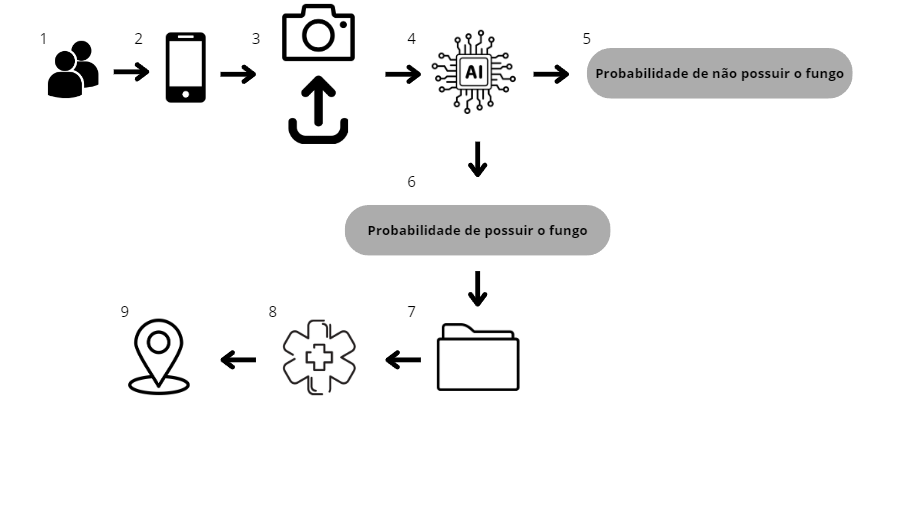
\includegraphics[width = \CaptionWidth]{Illustrations/Metodologia.png}}
  \usebox0%
  \SourceOrNote{Autoria Própria (2024)}
  \end{photograph}
Imagem 1 e 2: O usuário acessa o aplicativo e realiza o seu cadastro fornecendo as informações pessoais básicas. Esse cadastro é necessário para o uso das funcionalidades do sistema e para o armazenamento dos dados do usuário

Imagem 3 : Após o login, o usuário interage com uma das interfaces do sistema que permite o acesso a câmera do dispositivo, ou o upload de alguma foto que esteja na galeria do mesmo. Essa imagem será utilizada na análise da presença do fungo no tronco ou raiz da árvore

Imagem 4: Após o upload ou da captura da imagem, o sistema de inteligência artificial processa a imagem e calcula a probabilidade da presença do fungo Phytophthora 

Imagem 5: Caso a probabilidade do fungo ser baixa, o sistema informará o usuário que a árvore está saudável e que não precisa de cuidados além dos necessários, o que indicará também o sucesso do sistema

Imagem 6: Se a probabilidade do fungo indicar como elevada, o aplicativo emitirá um alerta ao usuário sobre a presença da infecção

Imagem 7: Em caso da doença, a imagem será armazenada em uma aba do aplicativo onde o usuário poderá informar a localização da árvore.

Imagem 8: O sistema indicará o que fazer com a árvore e quais são os cuidados necessários para com a mesma

Imagem 9: O aplicativo então armazenará a imagem no banco de dados e caso seja necessário o usuário terá acesso as fotos, que estarão disponíveis em outra aba do aplicativo, e terá acesso a localização da árvore em seu pomar. \label{sect:metodologia}

\input{Topicos/metodologia}

\section*{RESULTADOS PRELIMINARES}Os resultados preliminares obtidos são os protótipos das telas do aplicativo mobile e do Apex, as imagens a seguir mostram o desenvolvimento dos mesmos

\section*{Figma}
Nesta seção serão apresentados os resultados da prototipação no figma e do apex

Na img.1 é demonstrada a tela inicial do aplicativo onde o usuário é redirecionado para a tela
de login

\begin{figure}[H]
    \centering
    \caption*{Figma}
    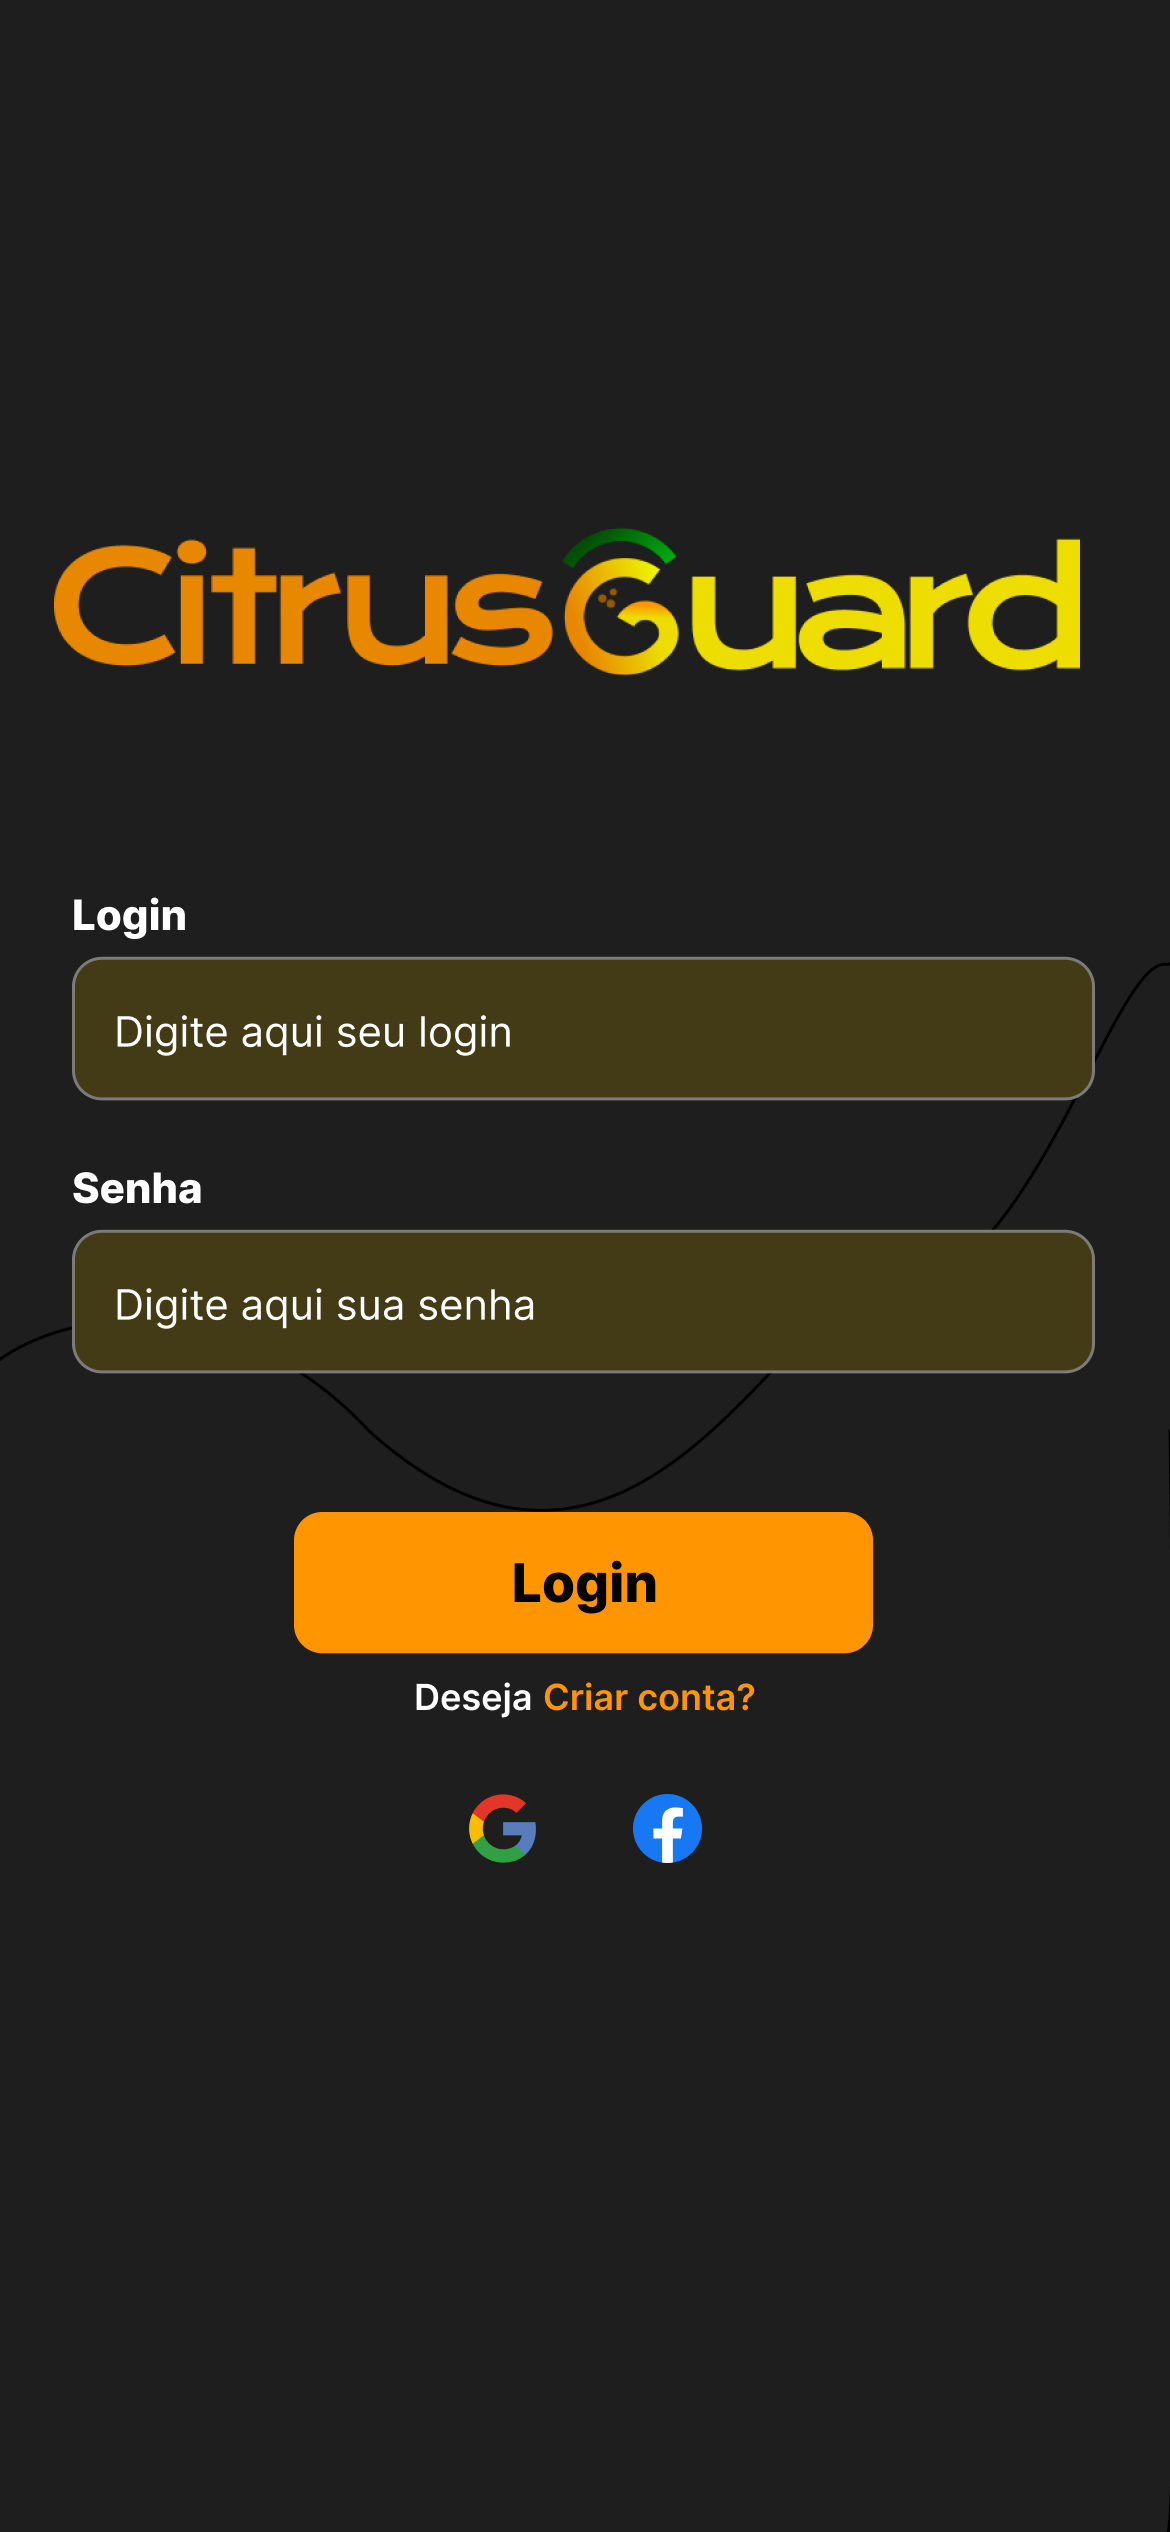
\includegraphics[width=5cm,height=10cm]{Illustrations/figma1.png}
    \caption*{Fonte: Figma (2024)}
    \label{fig:enter-label}
\end{figure}

A img.2 demonstra a tela inicial do aplicativo após o login ou cadastro do usuário

\begin{figure}[H]
    \centering
    \caption*{Figma}
    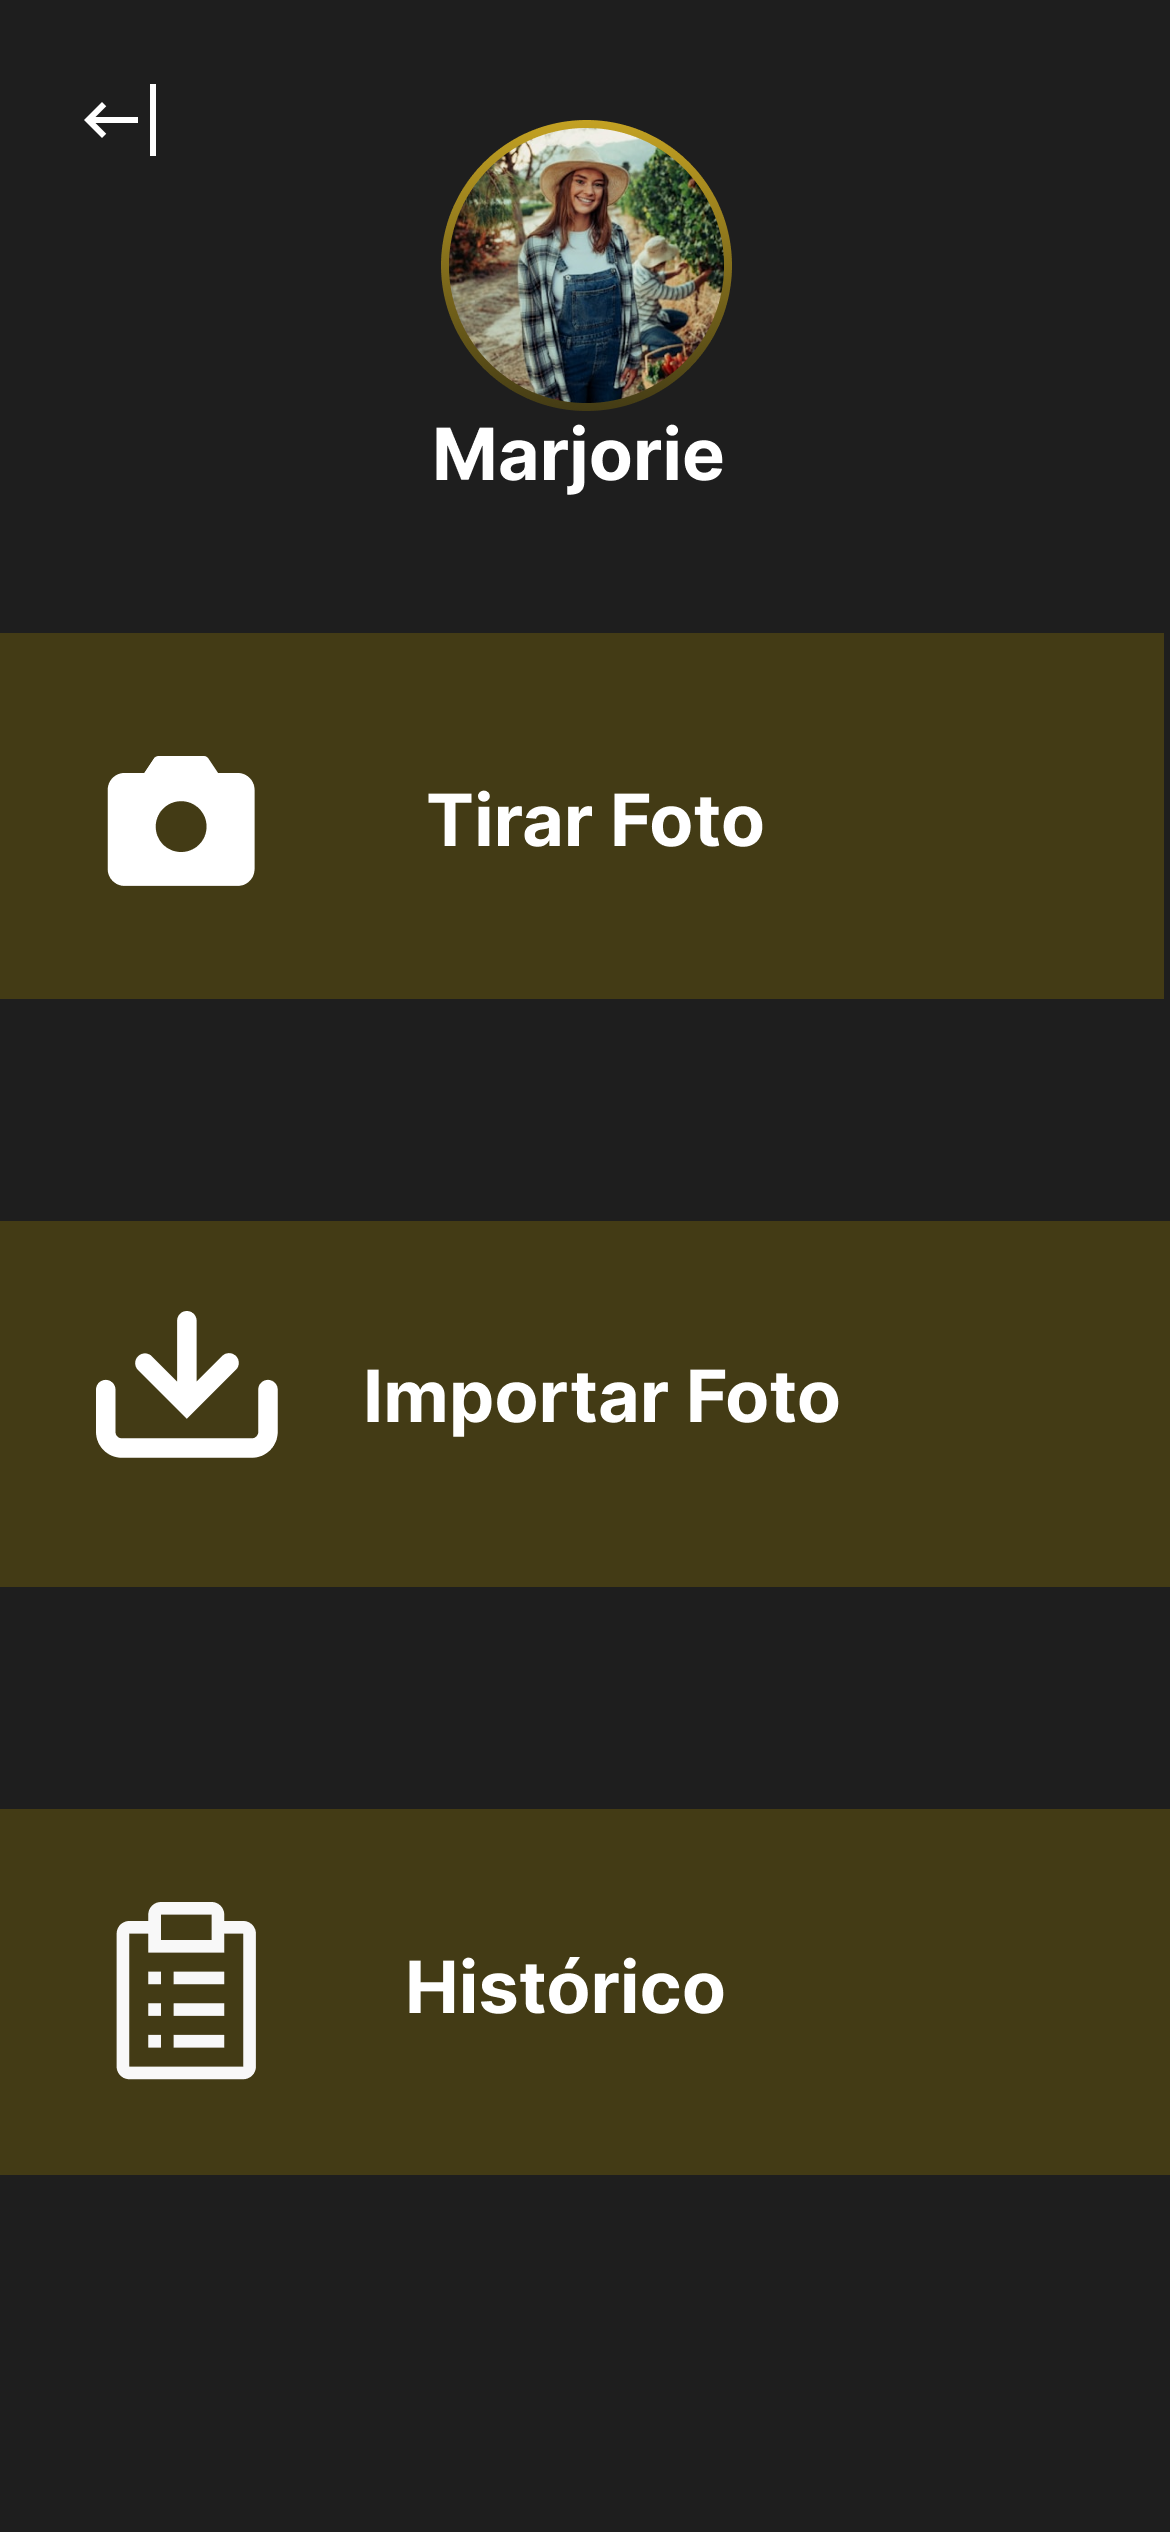
\includegraphics[width=5cm,height=10cm]{Illustrations/figma2.png}
    \caption*{Fonte: Figma (2024)}
    \label{fig:fig2}
\end{figure}

Na img.3 é possivel ver a galeria do usuário onde ele pode selecionar as fotos que desejar para a inteligência artificial analisar a imagem

\begin{figure}[H]
    \centering
    \caption*{Figma}
    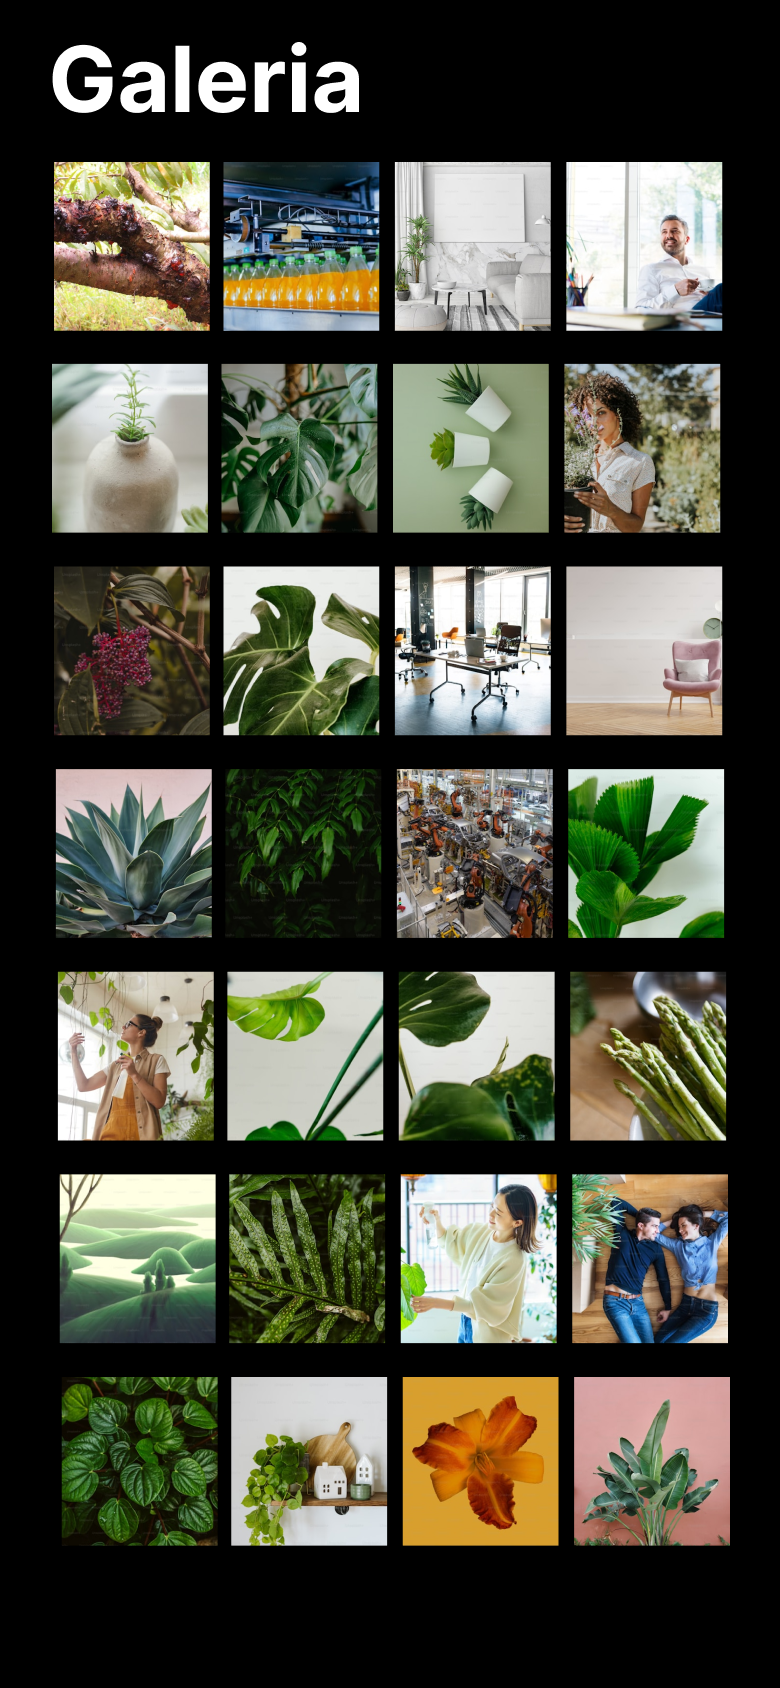
\includegraphics[width=5cm,height=10cm]{Illustrations/figma3.png}
    \caption*{Fonte: Figma (2024)}
    \label{fig:fig3}
\end{figure}

Com a imagem selecionada, a inteligência artificial então começa a fazer a análise como demonstrado abaixo

\begin{figure}[H]
    \centering
    \caption*{Figma}
    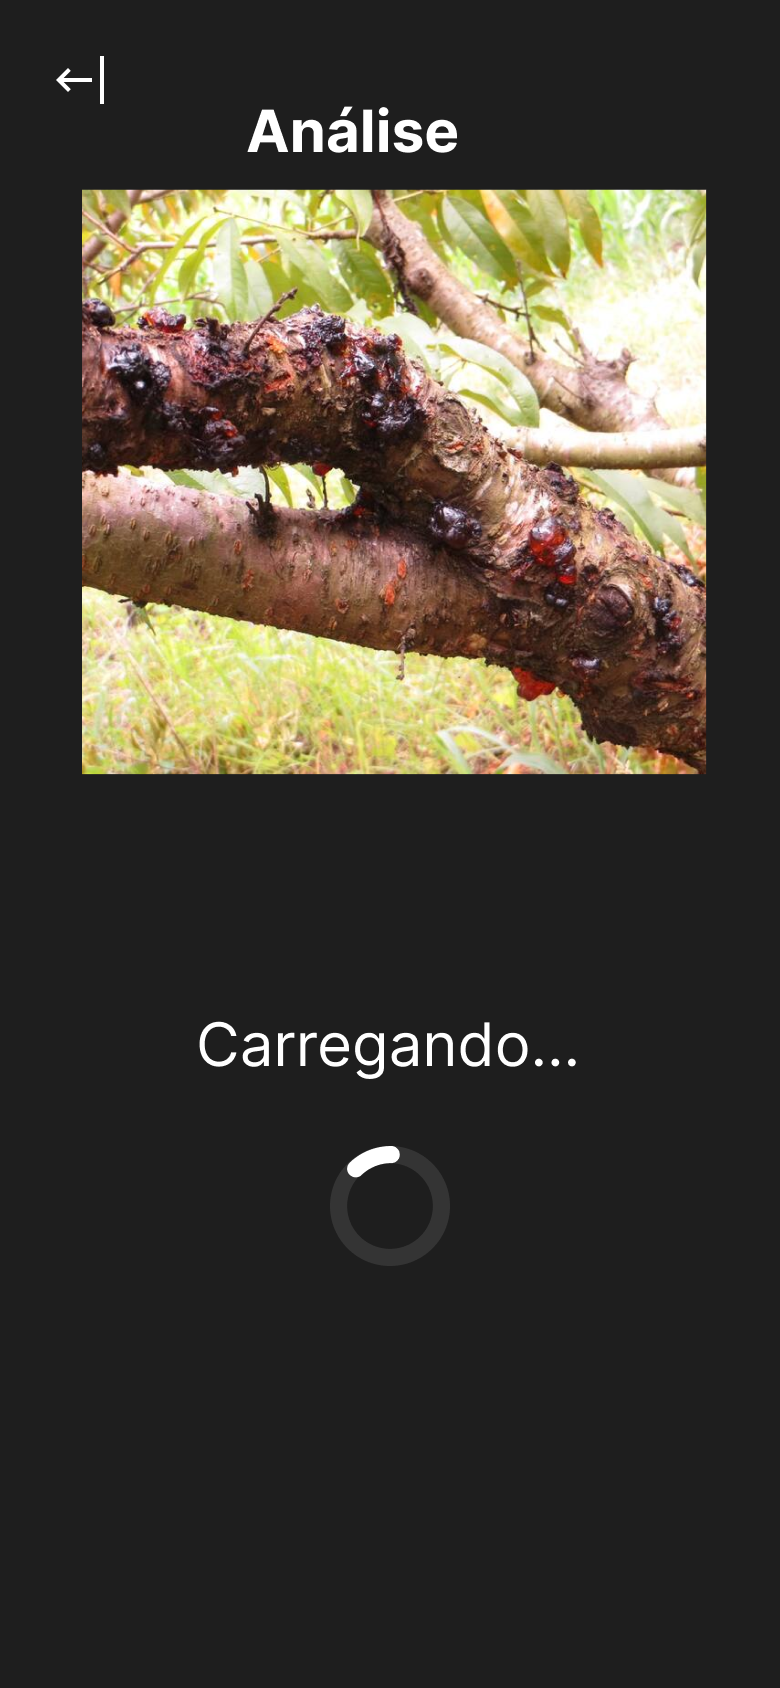
\includegraphics[width=5cm,height=10cm]{Illustrations/figma4.png}
    \caption*{Fonte: Figma (2024)}
    \label{fig:fig4}
\end{figure}

Na img.5 a IA já terminou de fazer a análise da probabilidade da gomose dentro do tronco e da o resultado em porcentagem para o usuário  

\begin{figure}[H]
    \centering
    \caption*{Figma}
    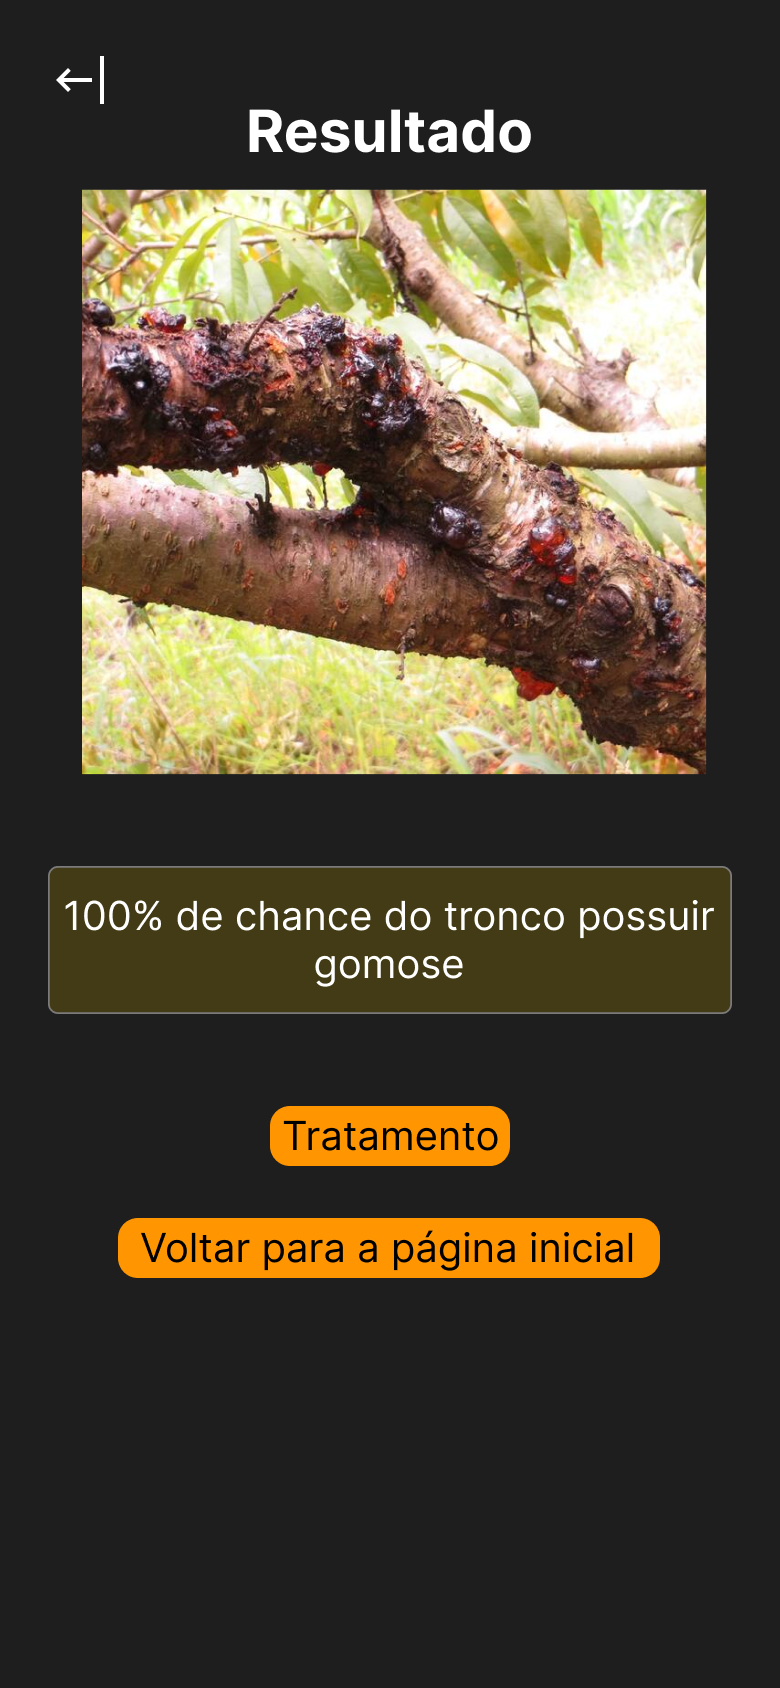
\includegraphics[width=5cm,height=10cm]{Illustrations/figma5.png}
    \caption*{Fonte: Figma (2024)}
    \label{fig:fig5}
\end{figure}

Com a planta infectada, o usuário pode escolher ver os tratamentos existentes para a planta clicando no botão "Tratamento"

\begin{figure}[H]
    \centering
    \caption*{Figma}
    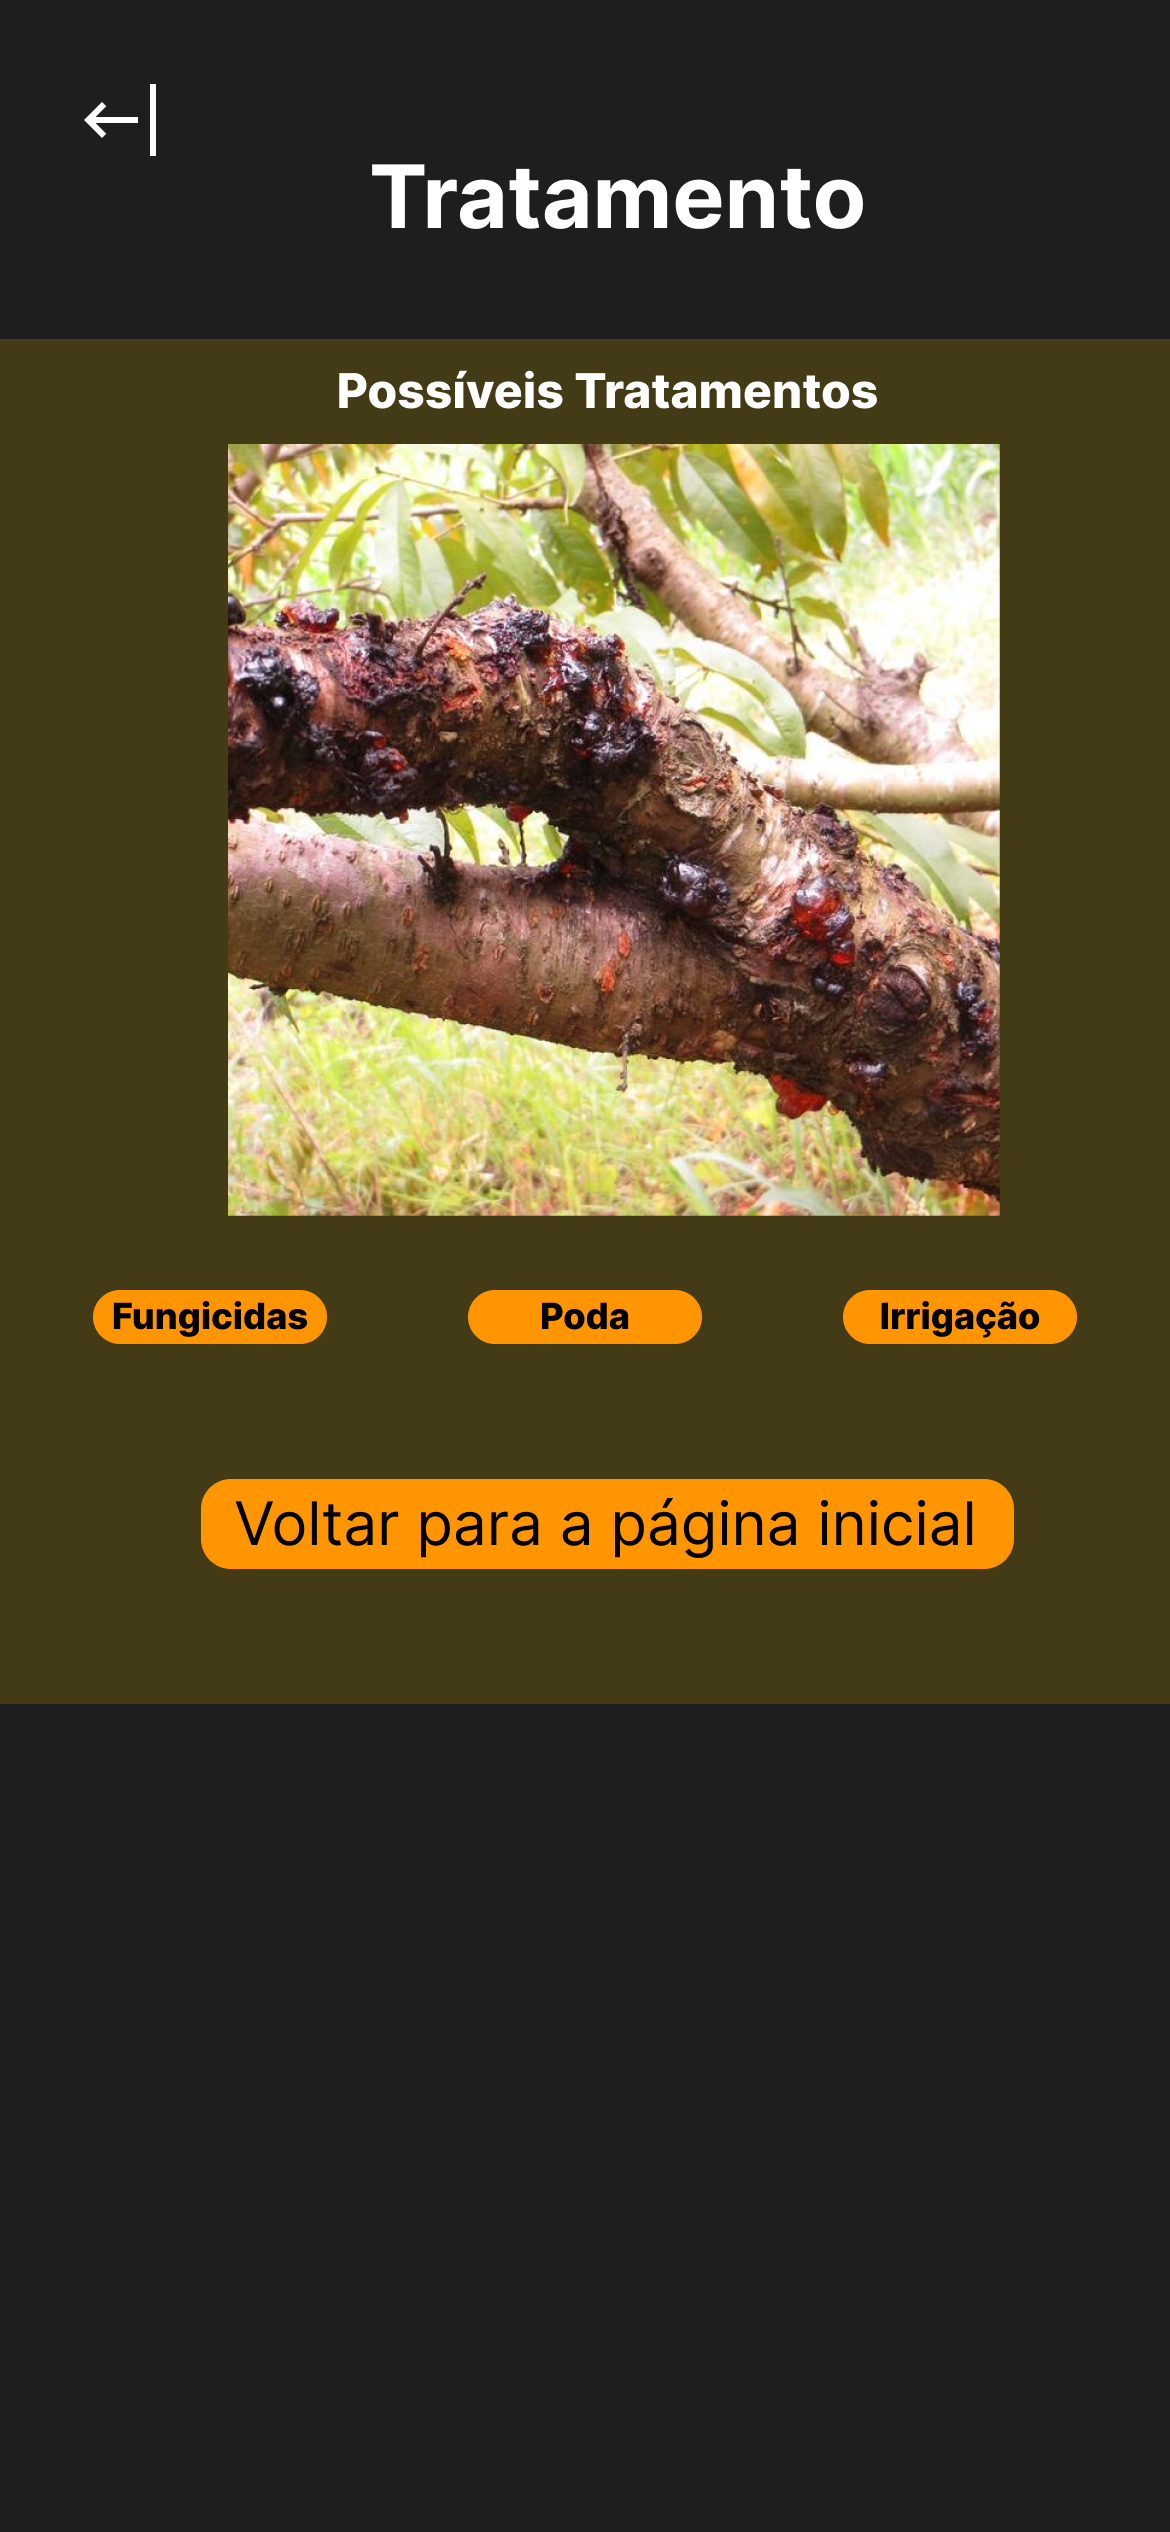
\includegraphics[width=5cm,height=10cm]{Illustrations/figma6.png}
    \caption*{Fonte: Figma (2024)}
    \label{fig:fig6}
\end{figure}

Os tratamentos ideais então serão mostrados ao usuário, conforme a imagem 7

\begin{figure}[H]
    \centering
    \caption*{Figma}
    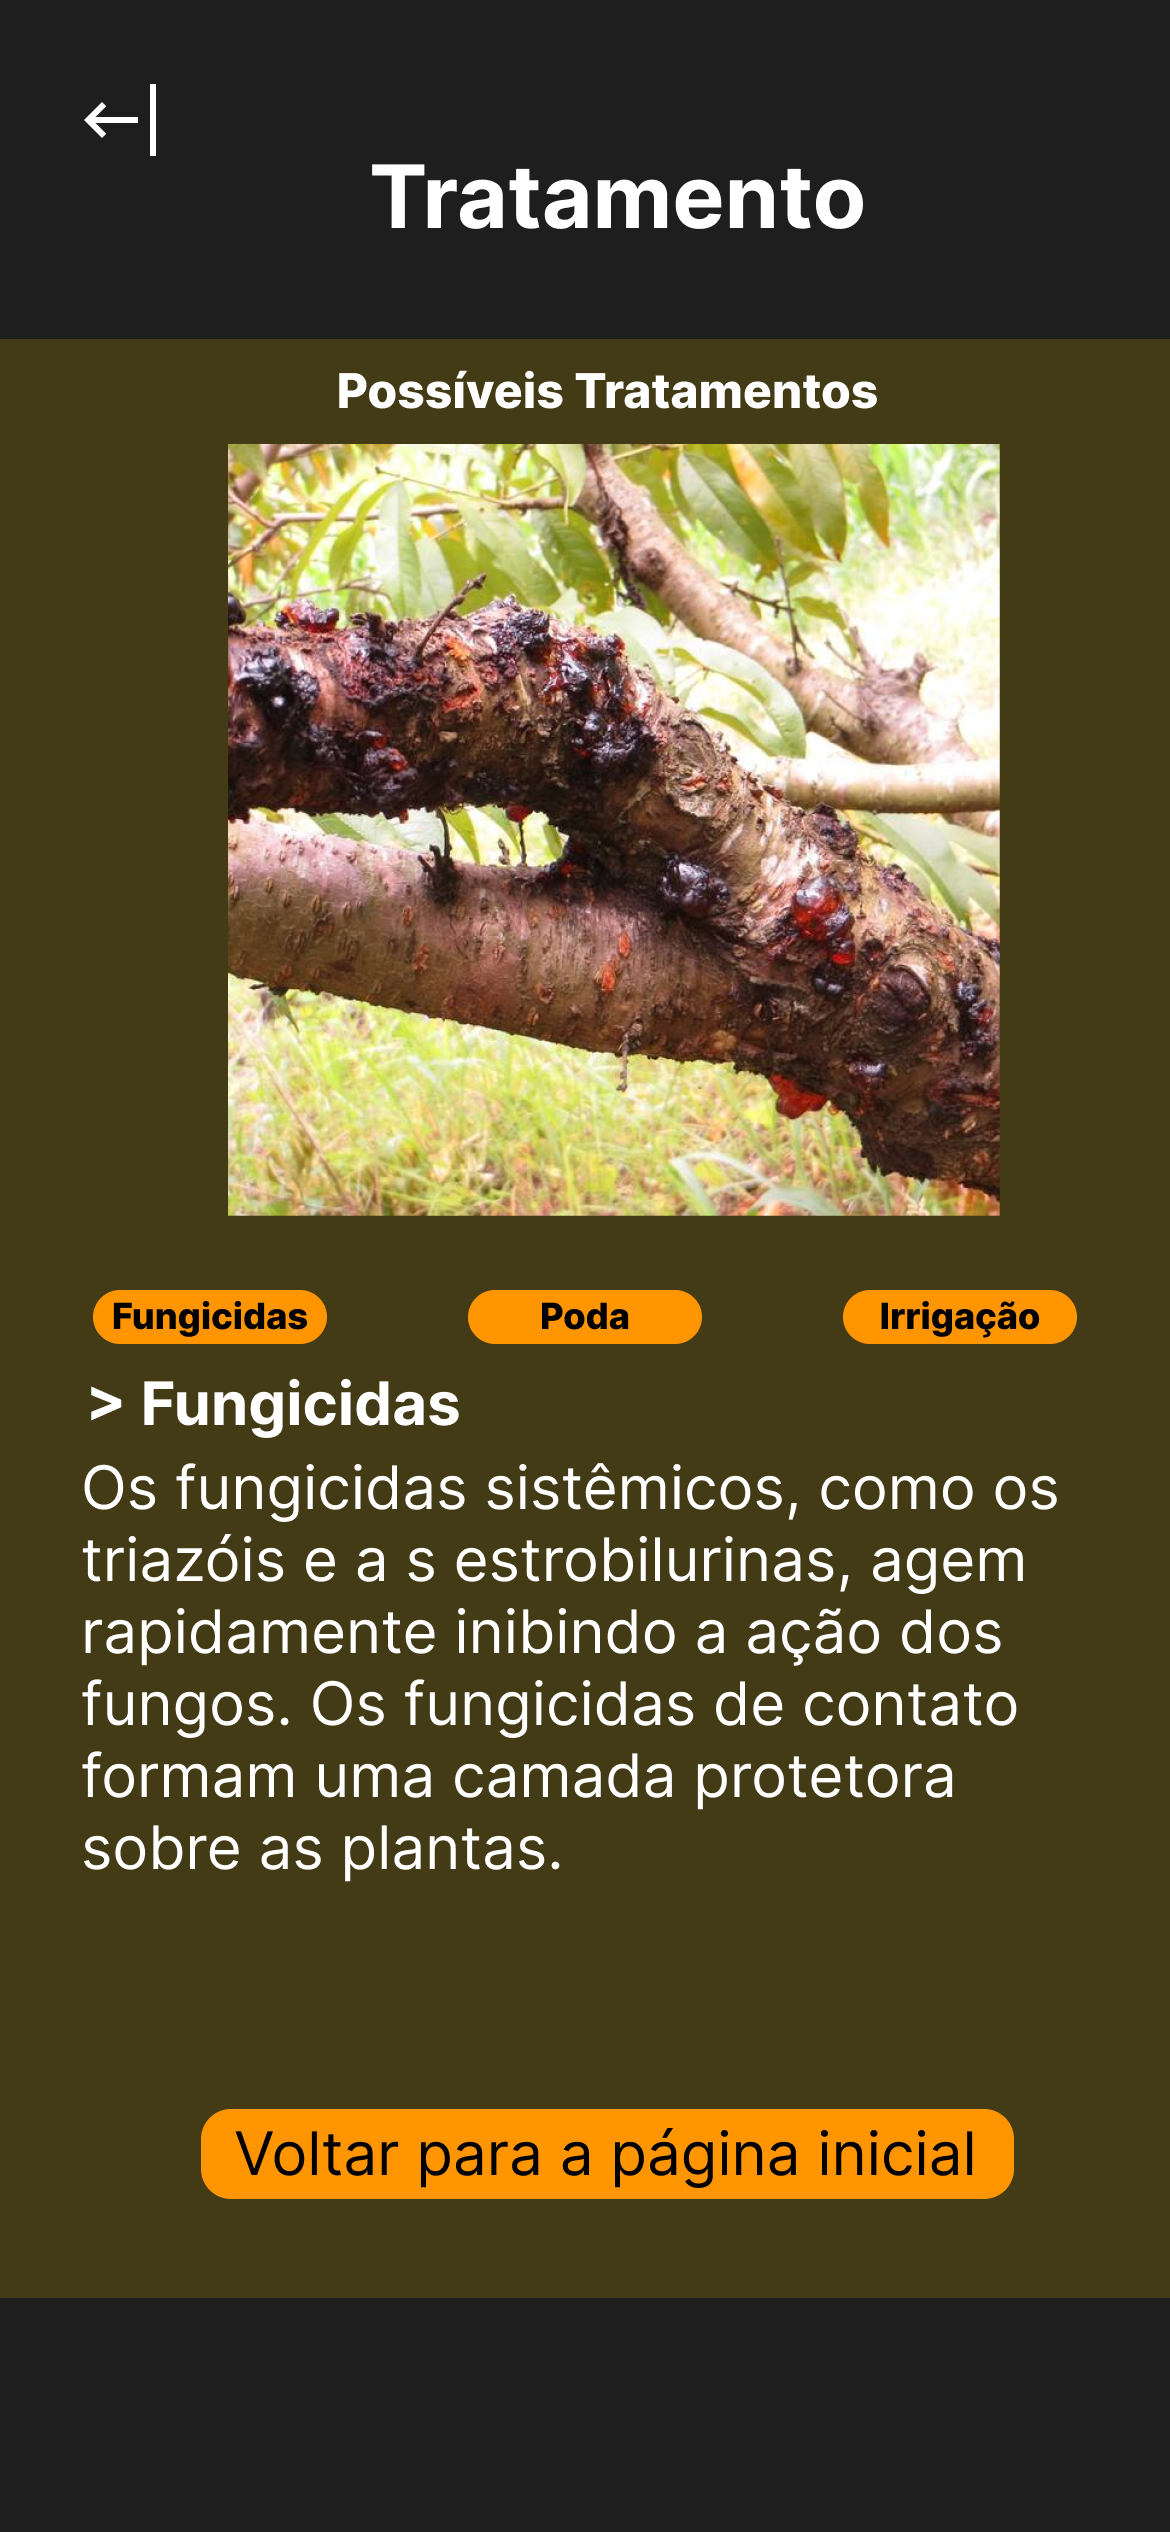
\includegraphics[width=5cm,height=10cm]{Illustrations/figma7.png}
    \caption*{Fonte: Figma (2024)}
    \label{fig:fig7}
\end{figure}

O usuário também terá acesso a uma aba de histórico, onde será possivel ver todas as plantas na qual ele tirou foto ou deu upload da sua galeria

\begin{figure}[H]
    \centering
    \caption*{Figma}
    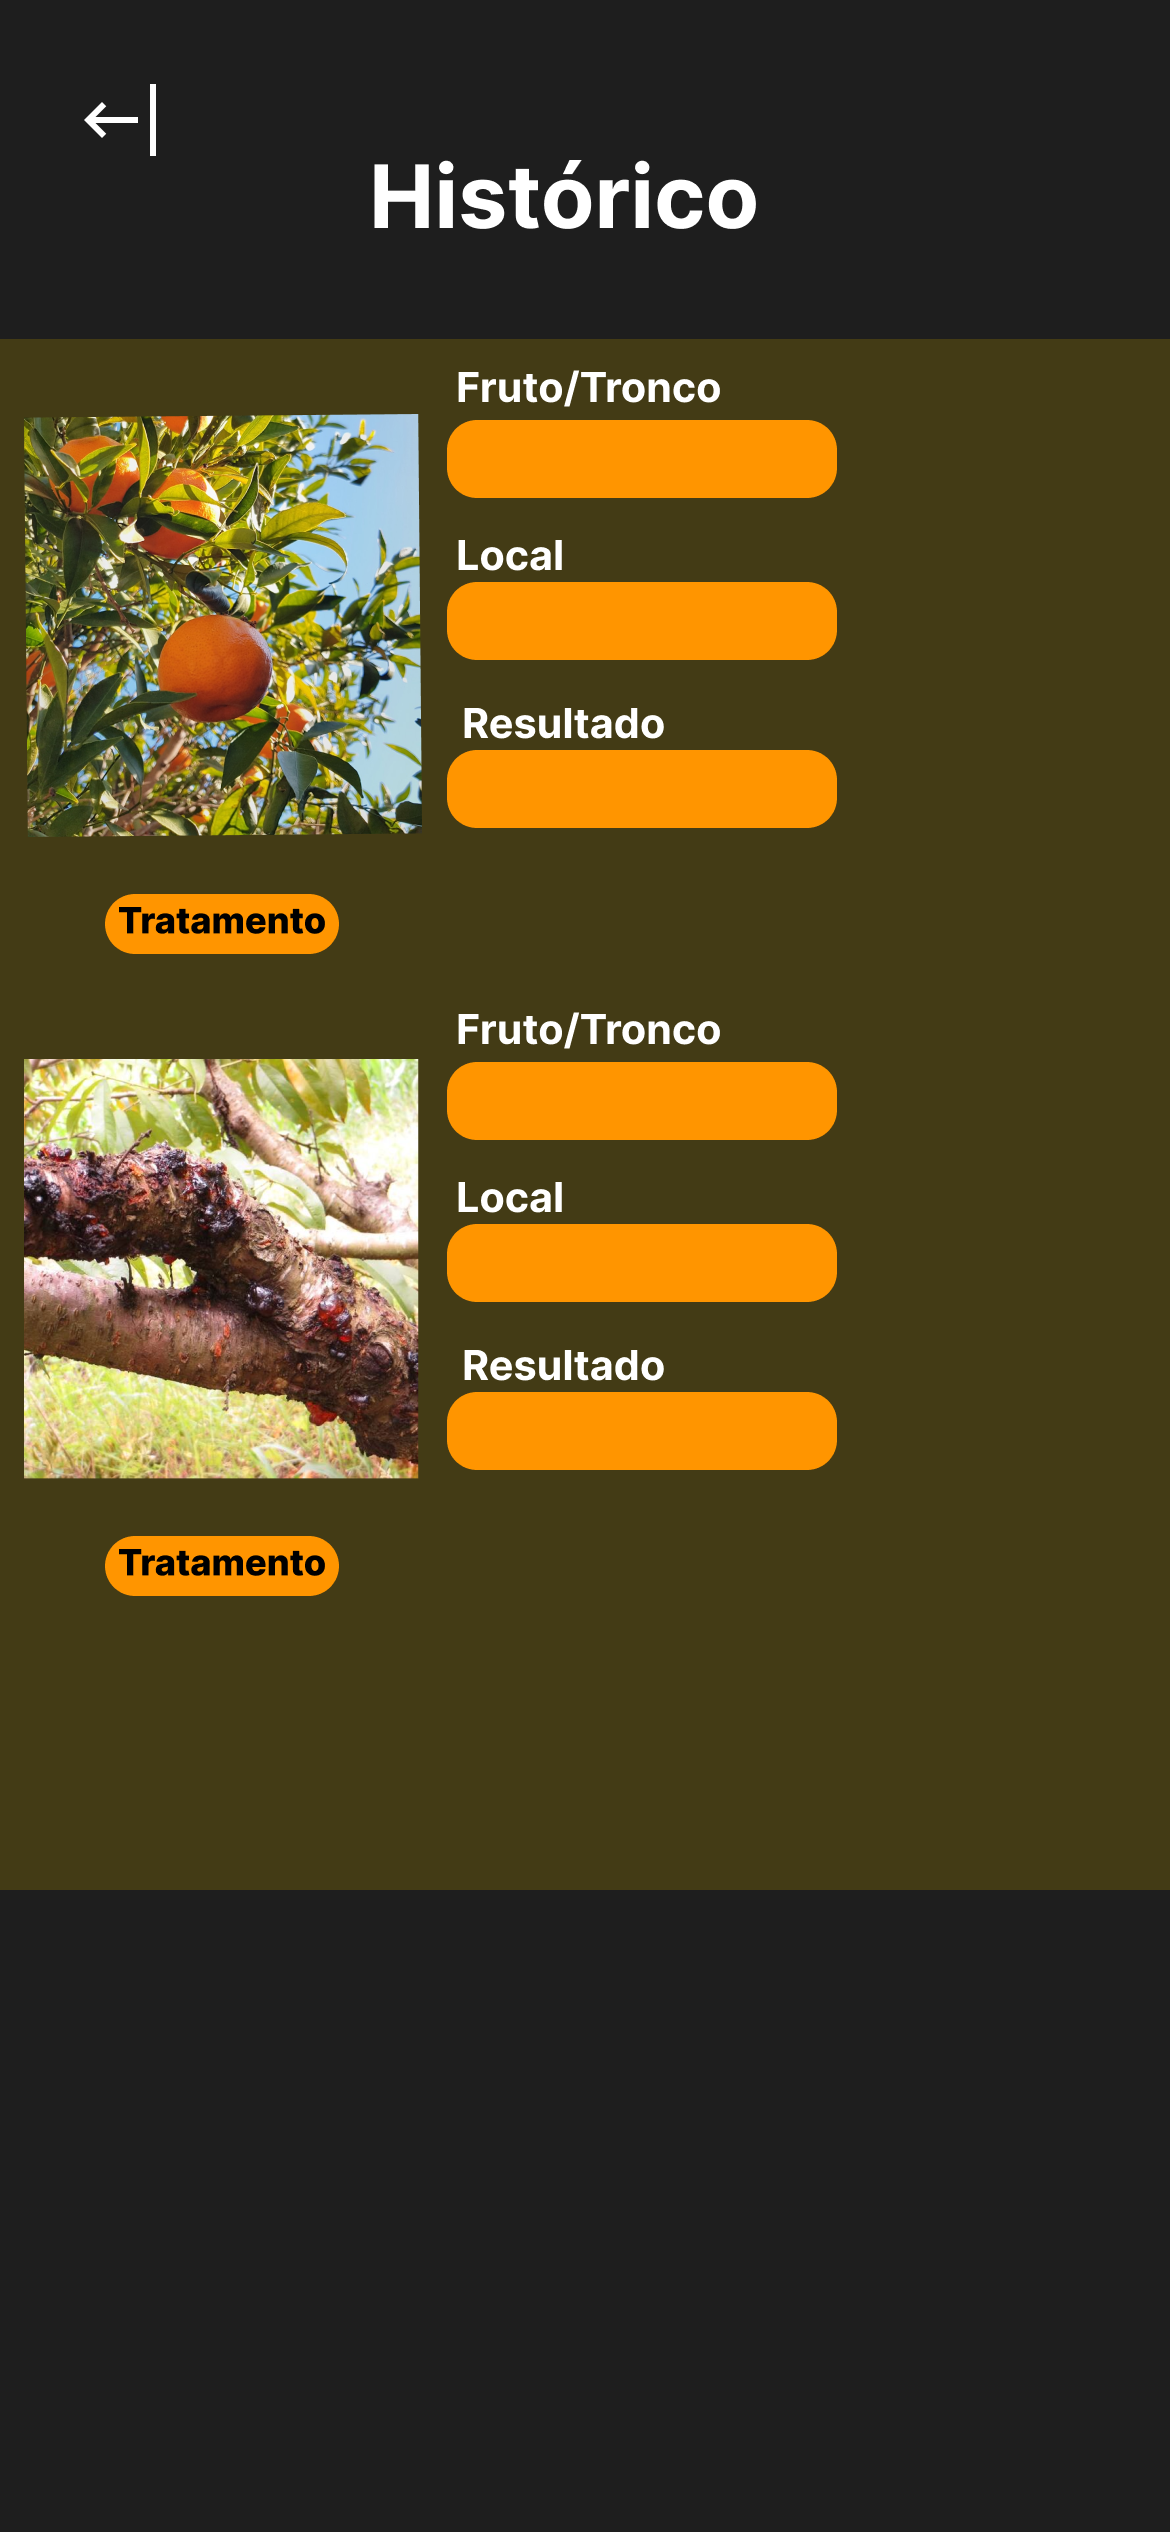
\includegraphics[width=5cm,height=10cm]{Illustrations/figma8.png}
    \caption*{Fonte: Figma (2024)}
    \label{fig:fig8}
\end{figure}

Na aba de histórico, também é possivel adicionar data, local, o nome do fruto ou tronco e uma descrição breve de qual o tratamento realizado com a planta 

\begin{figure}[H]
    \centering
    \caption*{Figma}
    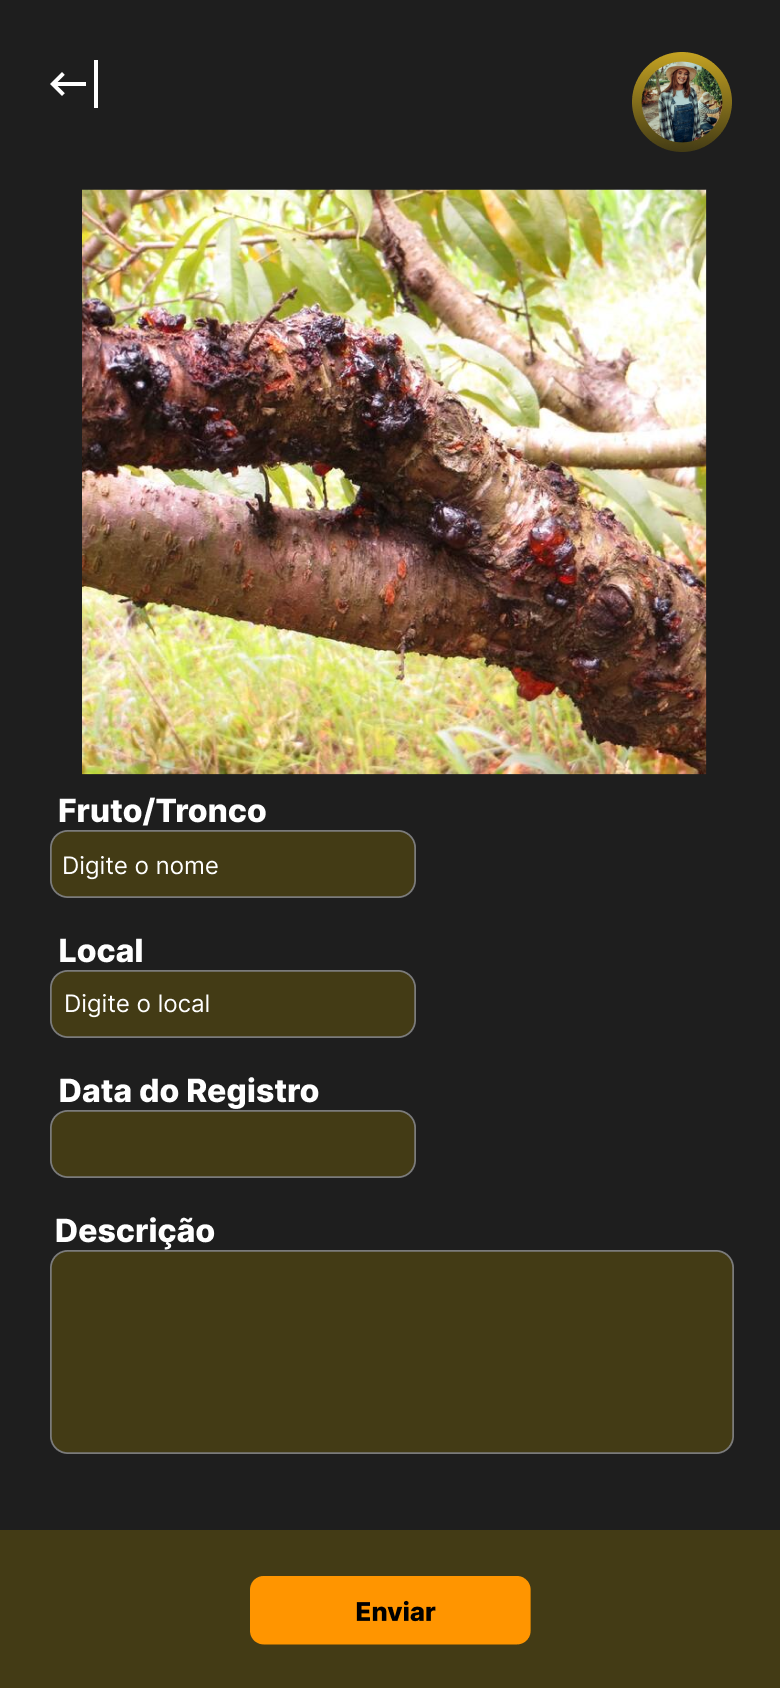
\includegraphics[width=6cm,height=11cm]{Illustrations/figma9.png}
    \caption*{Fonte: Figma (2024)}
    \label{fig:fig9}
\end{figure}

\section*{Apex}

O apex a seguir contem o banco de dados do aplicativo e as funcionalidades de localização do fruto ou tronco

Na img.1 podemos ver a tela de login do apex, contendo o email e senha para o acesso ser garantido 

\begin{figure}[H]
    \centering
    \caption*{Apex}
    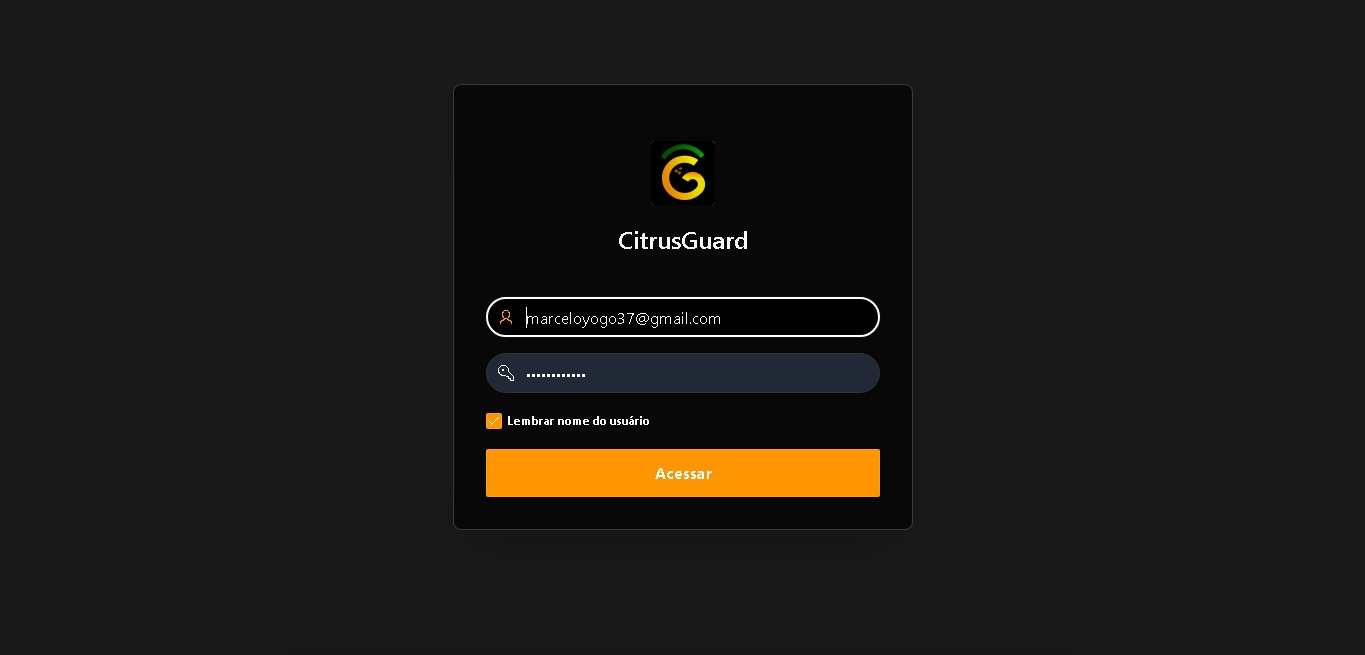
\includegraphics[width=14cm,height=8cm]{Illustrations/APEX1.jpg}
    \caption*{Fonte: Oracle Apex (2024)}
    \label{fig:apex1}
\end{figure}

Na img.2 do apex é possivel ver a tela inicial, a importação das fotos e a localização das plantas

\begin{figure}[H]
    \centering
    \caption*{Apex}
    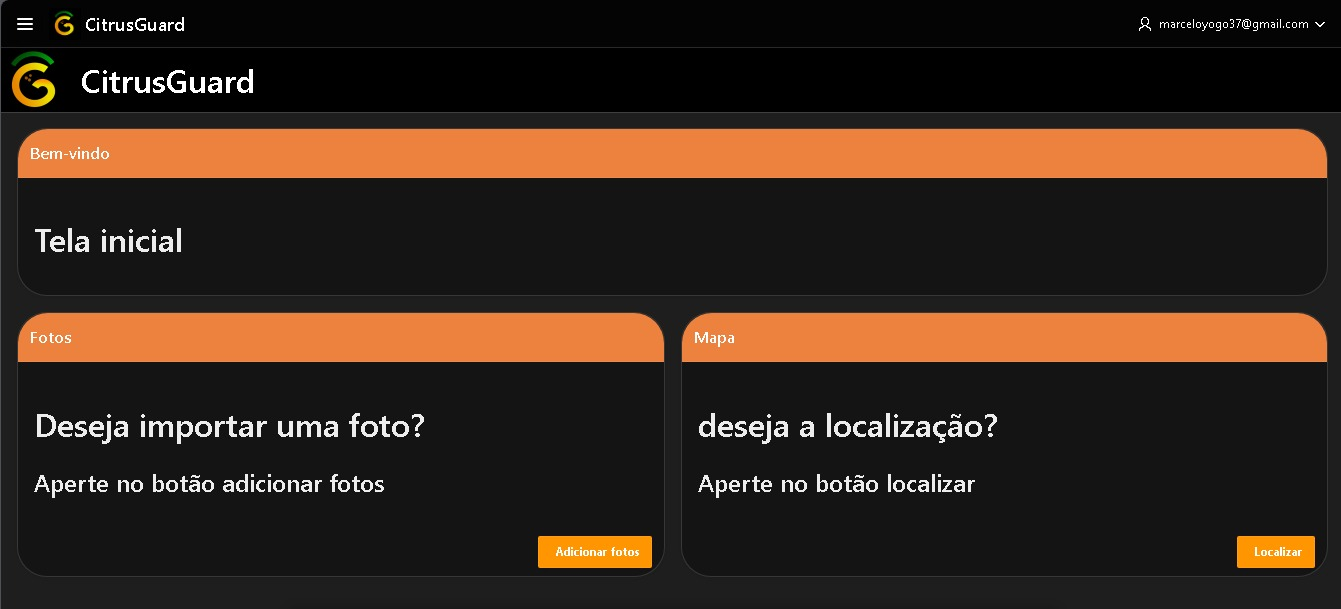
\includegraphics[width=14cm,height=8cm]{Illustrations/APEX2.jpg}
    \caption*{Fonte: Oracle Apex (2024)}
    \label{fig:apex2}
\end{figure}

A img.3 do apex demonstra a localização de cada fruto cadastrado no aplicativo

\begin{figure}[H]
    \centering
    \caption*{Apex}
    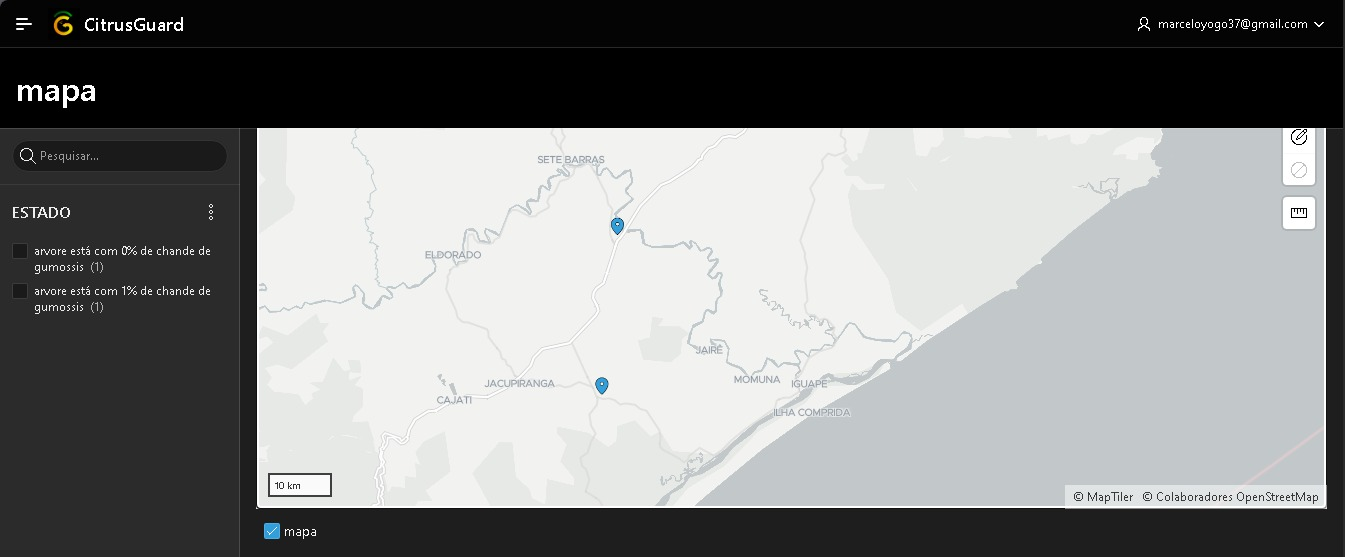
\includegraphics[width=14cm,height=8cm]{Illustrations/APEX3.jpg}
    \caption*{Fonte: Oracle Apex (2024)}
    \label{fig:apex3}
\end{figure}\label{sect:resultados}

\input{Topicos/resultados}

\section*{CONCLUSÃO}Este artigo tem como objetivo argumentar que é possível o uso da IA no meio agrícola. A Visão Computacional é um método de fácil programação e demonstra ser uma ferramenta muito eficaz para lidar com múltiplos dados. Com base nos artigos vistos anteriormente, sabe-se que a criação de aplicativos para a detecção, seja de doenças ou de espécies, é possível e que a IA traz probabilidades precisas. A Visão Computacional e o Deep Learning  são técnicas acessíveis e de fácil implementação que facilita a análise de grande volume de imagens lidando com a demanda dos agricultores com o cuidado de diversas plantas simultaneamente. O desenvolvimento de aplicativos, programas e sistemas baseados em IA vem aumentando o que torna essa tecnologia mais acessível a pequenos e grandes produtores, ajudando a prevenir surtos de doenças e a otimizar o uso de pesticidas. Em resumo, a integração com IA com visão computacional e com o Deep Learning no meio da agricultura e do agronegócio é viável e tem a tendência a crescer.
\label{sect:conclusao}

\input{Topicos/conclusao}

\printbibliography

%% Elementos pós-textuais (opcionais): Apêndice e Anexo
%Caso for utilizar, basta retirar o símbolo de % na frente do comando
%%%%% Elementos pós-textuais
%%
%% Glossário, apêndices, anexos e índice remissivo (opcionais).

%% Apêndices
\begin{Appendix}

\section{Título de Apêndice}%
\label{sect:apx-a1}

Exemplo de apêndice (\Cref{sect:apx-a1}) em uma seção de \nameref{sect:appendix}.

\subsection{Título de Seção Secundária de Apêndice}%
\label{ssect:apx-a2}

Exemplo de seção secundária de apêndice (\Cref{ssect:apx-a2}).

\subsubsection{Título de Seção Terciária de Apêndice}%
\label{sssect:apx-a3}

Exemplo de seção terciária de apêndice (\Cref{sssect:apx-a3}).

\paragraph{Título de seção quaternária de Apêndice}%
\label{prgh:apx-a4}

Exemplo de seção quaternária de apêndice (\Cref{prgh:apx-a4}).

\subparagraph{Título de seção quinária de Apêndice}%
\label{sprgh:apx-a5}

Exemplo de seção quinária de apêndice (\Cref{sprgh:apx-a5}).

\end{Appendix}

%% Anexos
\begin{Annex}

\section{Título de Anexo}%
\label{sect:anx-a1}

Exemplo de anexo (\Cref{sect:anx-a1}) em uma seção de \nameref{sect:annex}.

\subsection{Título de Seção Secundária de Anexo}%
\label{ssect:anx-a2}

Exemplo de seção secundária de anexo (\Cref{ssect:anx-a2}).

\subsubsection{Título de Seção Terciária de Anexo}%
\label{sssect:anx-a3}

Exemplo de seção terciária de anexo (\Cref{sssect:anx-a3}).

\paragraph{Título de seção quaternária de Anexo}%
\label{prgh:anx-a4}

Exemplo de seção quaternária de anexo (\Cref{prgh:anx-a4}).

\subparagraph{Título de seção quinária de Anexo}%
\label{sprgh:anx-a5}

Exemplo de seção quinária de anexo (\Cref{sprgh:anx-a5}).

\end{Annex}

%% Índice remissivo
\printindex%


%% Fim do documento
\end{document}